\documentclass{sig-alternate}

%\documentclass{article}
\usepackage[subpreambles=false]{standalone}


\usepackage{csquotes}
\usepackage{amsmath}

\usepackage[all=normal,
paragraphs=tight,
floats=tight,
%mathspacing=tight,
%wordspacing=tight,
tracking=tight,
bibbreaks=tight]{savetrees}
\usepackage{microtype}
\usepackage{adjustbox}
\usepackage{flushend}

\usepackage{booktabs, array} % Generates table from .csv
\usepackage{pgfplots, pgfplotstable}


\pgfplotsset{
compat=1.12,
/pgfplots/table/search path={.,..,../data}
}

%\usepackage[dvipsnames]{xcolor}
\usepackage{tikz}
\usetikzlibrary{positioning}
\usetikzlibrary{shapes} 
\usetikzlibrary{arrows.meta}
\usetikzlibrary{decorations.pathmorphing}


\tikzset{
	tripleinner/.style args={[#1] in [#2] in [#3]}{
		#1,preaction={preaction={draw,#3},draw,#2}
	},
	triple/.style={%
		tripleinner={[line width=0.5pt,black] in
			[line width=3pt,white] in
			[line width=4pt,black]}	 
	}
}

\tikzset{
	input/.style={
		%circle,
		%draw,
		%Blue,
		minimum width = 2
	},
	datastore/.style={cylinder,
		draw,
		%Green,
		minimum width = 2
	},
	proc/.style={rectangle,
		draw,
		%Red,
		minimum size = 50
	},
	link/.style={->,
		black},
	multi/.style={-Implies,
		triple,
	},
	labe/.style={
		%Blue,
		fill=white,
		fill opacity=0.6,
		text opacity=1,
		font={\footnotesize\itshape}	
	}
}


\usepackage[backend=bibtex,
style=trad-abbrv,url=false, doi=false,
sorting=none, sortcites=true, hyperref=false]{biblatex}
\bibliography{master}

\usepackage[author={Lyndon White}]{pdfcomment}
\usepackage{cleveref}

\newcommand{\W}{\mathcal{W}}
\renewcommand{\c}{\mathbf{c}}
\newcommand{\s}{\mathbf{s}}
\renewcommand{\l}{\mathbf{l}}
\renewcommand{\u}{\mathbf{u}}
\newcommand{\ci}{\perp\!\!\!\perp} % from Wikipedia
\DeclareMathOperator*{\argmin}{arg\,min}
\DeclareMathOperator*{\argmax}{arg\,max}




\begin{document}

\title{Finding Word Sense Embeddings Of Known Meaning}

\numberofauthors{4}
\author{
	\alignauthor Lyndon White\\
	%\affaddr{School of Electrical, Electronic and Computer Engineering}\\
	\affaddr{University of Western Australia}\\
	\email{lyndon.white@research.uwa.edu.au}
	%
	\alignauthor Roberto Togneri\\
	%\affaddr{School of Electrical, Electronic and Computer Engineering}\\
	\affaddr{University of Western Australia}\\
	\email{roberto.togneri@uwa.edu.au}
	%
	\alignauthor Wei Liu\\
	%\affaddr{School of Computer Science and Software Engineering}\\
	\affaddr{University of Western Australia}\\
	\email{wei.liu@uwa.edu.au}
	%
	\and
	%
	\alignauthor Mohammed Bennamoun\\
	%\affaddr{School of Computer Science and Software Engineering}\\
	\affaddr{University of Western Australia}\\
	\email{mohammed.bennamoun@uwa.edu.au}
} 
%There are instructions about shared affilations on https://www.acm.org/sigs/publications/sigfaq#a17

\maketitle

\begin{abstract}
Word sense embeddings are vector representations of polysemous words -- words with multiple meanings. Similar techniques to those used to find word embedding vectors, such as in Word2Vec, are often used to learn multiple sense embeddings for each word.
These induced sense embeddings, however, do not necessarily correspond to any dictionary senses of the word.
This limits the applicability of these embeddings in traditional semantic-orientated tasks such as lexical word sense disambiguation.
To overcome this, we propose a method to find new sense embeddings of known meaning.
We term this method refitting, as the new embedding is fitted to model the meaning of a target word in the example sentence. The refitting is accomplished using probabilities of the existing induced sense embeddings, as well as their vector values.

Our contributions are threefold:
(1) The refitting method to find the new sense embeddings;
 (2) a novel smoothing technique, for use with the refitting method;
and (3) a new similarity measure for words in context, defined by using these refitted sense embeddings.

We show how our refitting based techniques improve the performance of the Adaptive Skip-Gram sense embeddings for word similarly evaluation; and how it allows the embeddings to be used for lexical word sense disambiguation -- which was not possible before refitting the sense embeddings.
Further to this, the similarity measure we derive from the refitting has significantly better time-complexity than the commonly used AvgSimC; making this more a more suitable method for large scale web-scale datasets.
\end{abstract}


\section{Introduction}


Word embeddings represent a word's semantic meaning and syntactic role as a point in a vector space \parencite{NPLM, collobert2008unified, mikolov2013efficient}. However, each word is only given one embedding -- which restricts it to representing only one combined sense. Word sense embeddings are the generalisation of this to handle polysemous and homonymous  words. Often these word sense embeddings are learnt through unsupervised word sense induction \parencite{Reisinger2010,Huang2012,tian2014probabilistic, AdaGrams}. In these cases it is not possible to directly determine which meaning belongs to which embedding. Furthermore the induced senses are unlikely to directly match to any one human defined meaning at all; but rather will be more specific, more broad, or include the meanings of jargon not in common use.


It can be argued that many word sense induction (WSI) systems may capture better word senses than human lexicographers do manually, however this does not mean that induced senses can replace standard lexical senses. While the induced senses may cover the space of meanings more comprehensively, or with better granularity than the standard senses, there is a vast wealth of existing knowledge defined around lexical senses from various sense inventories. Methods to link induced senses to lexical senses allow this information to be unlocked.


We thus propose a method for using a single example of a word in context to synthesise a new embedding for that particular sense. We term this \emph{refitting} the induced senses, as it combines them to fit to the meaning in the example sentence. Our method allows us to use a single labelled example to produce a labelled sense embedding. This allows a shift from a representation that can only work within the system, to one that uses a standard sense, or a user defined sense, which can be used as part of a more complex knowledge engineering system. 

Refitting word sense vectors to match a lexicographical sense inventory, such as WordNet or a translator's dictionary, is possible if the sense inventory features at least one example of the target senses use. The new lexically refitted sense embedding can then be used for Word Sense Disambiguation (WSD). Applying WSD adds useful information to an unstructured document, allowing further processing methods to take advantage of this information. An application of this would be as part of a machine translation system. To properly translate a word, the correct sense should be determined, as different senses in the source language, often translate to entirely different words in the target language. Using WSD to add sense annotation to a document bridges between unstructured raw text data to sense annotated data allowing for further processing with systems that require this structure. The application of our method for WSD is discussed in \Cref{lexicalWSD}.

Beyond refitting to a standard lexical sense, refitting to a user provided example has applications in information retrieval. Consider the natural language query \enquote{Find me web-pages about banks as in \enquote{the river banks were very muddy.}}. By generating an embedding vector for that specific sense of ``banks'' from the example sentence, and generating one from use of the word in each retrieved document, we can approximate measuring distance in a semantic space. This allows for similarity ranking -- discarding irrelevant uses of the word. The method we propose, using our refitted embeddings, has lower time complexity than AvgSimC, the current state of the art alternative for measuring similarity of words in context. This is detailed in \Cref{RefittedSimVsAvgSimC}

Our refitting method synthesises a new sense vector using the existing induced word sense vectors and the language model.
The new vector is formed as an appropriately weighted sum of the original embeddings. A weighting of the induced sense vectors is determined using the language model and the example sentence.
The refitted vector approximately corresponds to the meaning given by the example sentence. 
Our refitting method is detailed in \Cref{refitting}.

We noted during refitting often a single induced sense would dominate the refitted sense representation. It is rare in natural language for the meaning to be so unequivocal. Generally, a significant overlap exists between the meaning of different lexical senses, and there is often a high level of disagreement when humans are asked to annotate a corpus \parencite{veronis1998study}. We thus would expect similar to hold automatically determining the appropriateness of the induced senses, as is done during refitting. Towards this end, we develop a smoothing method, which we call \emph{geometric smoothing} that de-emphasises the sharp decisions made by the (unsmoothed) refitting method. We found that this significantly improves results. This suggests that the sharpness of decisions from the language model is an issue with the language model, which smoothing can correct. The geometric smoothing method is presented in \Cref{smoothing}.


We demonstrate the refitting method on Adaptive Skip-Grams (AdaGram) \parencite{AdaGrams}, and on our own simple greedy word sense embeddings. The method is applicable to any skip-gram-like language model that can take a sense vector as its input, and can output the probability of a word appearing in that sense's context.


The rest of the paper is organised as follows: \Cref{relatedwords} discusses related works on learning standard lexical sense repressions directly, and on associating the induced senses with standard lexical senses. \Cref{Framework} presents our refitting method, as well as the geometric smoothing method used with it. \Cref{lexicalWSD} shows how the refitted sense vectors can be used for lexical word sense disambiguation. \Cref{SimilarityInContext} describes the RefittedSim measure for word similarity in context, and presents its results. Finally, the paper presents its conclusions in \Cref{conclusion}.

\section{Related Works} \label{relatedwords}

\subsection{Directly Learning Lexical Sense Embeddings}
Our refitting method can be considered as learning lexical sense embeddings, as a one-shot learning task. A alternative is to transform the problem into a supervised or semi-supervised learning task. The difficulty lies in how to get a sufficient number of labelled senses. One option is to use a separate WSD method to artificially label an unlabelled corpus.

Iacobacci et al. \parencite{iacobacci2015sensembed} use a Continuous Bag of Word language model\parencite{mikolov2013efficient}, but use word senses as the labels rather than words. This is a direct application of word embedding techniques. To overcome the lack of a large sense labelled corpus, Iacobacci et al. use the 3rd party WSD tool BabelFly, to add sense annotations to a previously unlabelled corpus. An alternative approach would be to use a method that disambiguates the senses using a partially trained model.

Chen et al. use a semi-supervised approach to train sense vectors \parencite{Chen2014}. They partially disambiguate their training corpus, using their initial word sense vectors and WordNet; and use these labels to fine-turn their embeddings.
Initially the sense vectors are set as the average of the single sense word embeddings\parencite{mikolov2013efficient} for the words in the WordNet gloss.
Similarly, they define a context vector, as the average of all words in a sentence.
They then progressively label the words with the sense of the sense vector that is closest to the context vector if it is closer than a fixed threshold.
The requirement for meeting a threshold in order to add the sense label  decreases the likelihood of training on an incorrect sense label.
The selected sense vector is used to update the context vector and then the next word is relabelled. They give two methods for selecting the order of relabelling.
After the relabelling is complete they fine tune the sense embeddings by defining a new skip-gram method with the objective of predicting both the words and the word senses in the context, when given an input word\footnote{Note that using the input word to predict the which word senses will appear in the context is the opposite of the approach used by AdaGram. AdaGram uses the word sense to predict the word of the context \parencite{AdaGrams}.}. The overall approach is to use the initial sense vectors estimated from the glosses to add sense labels to some of the words, and then use these as the training target.

The key practical difference between the one-shot approach used by refitting, compared to the supervised, and semi-supervised approach uses in existing works is the time taken to  add a new sense. With our refitting fitting approach adding a new sense is practically instantiations, and replacing the entire sense inventory is only a matter of a few hours. Whereas for the existing approaches adding senses would require almost fully repeating the training process, often taking several days. Refitting is a process done to sense word embeddings, rather a method for finding sense embeddings from a large corpus. It can be applied to any pretrained sense embeddings, so long as it meets the requirement for a suitable language model.
\pdfcomment{Should I mention that it could be adapted to apply to both the embeddings above, with some adaption?}

One of the key reasons, that it is useful to have senses that align with standard lexical senses, is that it allows word sense embeddings to be used for word sense disambiguation. This is demonstrated by Chen et al.  \parencite{Chen2014}, and we discuss how refitted word sense vectors can be used do the same in \Cref{eq:lexicalwsd}. If the word senses do not correspond to the lexical senses, then one approach is to form a weighted mapping from induced senses, to the lexical senses.

\subsection{Mapping induced senses to lexical senses}\label{mapping}
 Agirre et al. give a general method to allow induced word senses to be used for lexical WSD \parencite{agirre2006}.
Their method applies to all word sense induction systems, not just word embedding systems, so is more general than the refitting approach that we present.
Their method maps the induced sense disambiguation scores, to scores for disambiguating standard lexical senses. This method was used for the SemEval-2007 Task 02 \parencite{SemEval2007WSIandWSD} to evaluate all entries.
They use an annotated \emph{mapping corpus} to construct a mapping weight between induced senses probabilities and the lexical sense probabilities.

For $\l=\{l_1,...\}$ the set of lexically defined senses, $\u=\{u_1,...\}$ the set of unsupervised induced senses, and a corpus of labelled contexts $\{\c_1, ...\}$ Agirre et al. define the mapping weight by a likelihood.
This likelihood $P(l_i \mid u_j)$ is estimated by counting how often $u_j$ is the most-likely sense as returned by WSD on the induced senses, when $l_i$ is the labelled lexical sense; and applying the definition of conditional probability.

This method requires the mapping corpus to cover every lexical word sense, with enough instances for the frequency count to converge to the actual likelihood.

This is used to disambiguate a target word within a sentence ($\c_T$)  by converting the the unsupervised sense score $P(u_j \mid \c_T)$ to supervised sense scores $P(l_j \mid \c_T)$ by
\begin{equation} \label{eq:agireewsd}
P(l_i \mid \c_T) = P(l_i | u_j) P(u_j \mid \c_T)
\end{equation}


Agirre et al. demonstrate this method with the small Senseval 3 English Lexical Sample \parencite{mihalcea2004senseval} -- it is less clear how well it will work on more complete tasks featuring rarer words and senses. We use this method as a baseline in \Cref{lexicalWSD}.


\section{Proposed Refitting Framework} \label{refitting} \label{Framework}

The key contribution of this work is to provide a way to synthesise a word sense embedding given only a single example. This is what we call this \emph{refitting} the sense vectors. By refitting the unsupervised vectors we define a new vector, that lines up with the specific meaning of the word from the example sentence.

This can be looked at as a one-shot learning problem.
The training of the induced sense, and of the language model, can be considered an unsupervised pre-training step. The new word sense embedding should give a high value for the likelihood of the example sentence, according to the language model. Furthermore, it should generalise to also give a high likelihood of other contexts that were never seen, but which also occur near the word sense of this particular meaning.

As part of our preliminary investigations, we attempted directly optimising the sense vector so as to maximise the probability of the example. This was found to generalise poorly, due to over-fitting. It also took a significant amount of time. Rather than a direct approach, we instead take inspiration from the locally linear relationship between meaning and vector position that has been demonstrated for (single sense) word embeddings \parencite{mikolov2013efficient,mikolovSkip,mikolov2013linguisticsubstructures}.

In order to refit the sense embedding to align to the meaning of the word in a particular context, we express it as a combination of the unsupervised sense vectors for that word.
The new sense vector is a weighted sum of the existing vectors that were already trained, where the weight is determined by the probability of each induced sense given the context.


Assume we are given a collection of induced (unlabelled) embeddings $\u={u_1,...,u_{n_u}}$, and an example sentence $\c={w_1,...,w_{n_c}}$. We define a function $l(\u \mid \c )$ which determines the refitted sense vector, from the unsupervised vectors and the context:

\begin{equation} \label{eq:synth}
l(\u \mid \c ) = \sum_{\forall u_i \in \u} u_i P(u_i \mid \c)
\end{equation}

To do this, we need to estimate the posterior predictive distribution $P(u_i \mid \c)$.
This can be done by using Bayes' Theorem, as shown in \Cref{generalwsd}; or with our smoothed variation discussed in \Cref{smoothing}


In the very first neural network language model paper, Bengio et al. \parencite{NPLM} describe a similar method to \Cref{eq:synth} for finding the word embeddings for words not found in their vocabulary. They suggest that if a word was not present in the training data, they form \enquote{an initial feature vector for such a word, by taking a weighted convex combination of the feature vectors of other words that could have occurred in the same context, with weights proportional to their conditional probability} \parencite{NPLM}. The formula they give is as per \Cref{eq:synth}, but summing over the entire vocabulary of words (rather than just $\u$). To the best of our knowledge, this method has not been used for handling out-of-vocabulary words in any more recent word embedding architectures, nor has it ever been used for sense vectors.


\subsection {Fall back for Dictionary Phrases (Collocations)}
Unless a specialised tokenizing method is used, a word embedding method will not learn embeddings for collocations such as ``civil war'' or ``martial arts''. Normal tokenizers will split these at the word level, learning embeddings for ``civil'', and ``war'', and for ``martial'' and ``arts''. This issue is often considered minimal for word embeddings, as an approximate embedding can be constructed by summing embeddings for each word in the phrase.

For single-sense word embeddings  summing the word embeddings of the words making up the phrase results in reasonable representation \parencite{mikolovSkip, White2015SentVecMeaning}.
As we are already creating a weighted sum, in the refitting step (\Cref{eq:synth}), we can facilitate a similar result by adding the additional sense embeddings for each word to the total pool of sense embeddings to be combined ($\u$ above). This allows for the senses of one word to contribute more than the other.

It is likely that one word in a collocation will contain senses with more specialised use in the collocation than the other.
For example, \enquote{civil war}: \enquote{war} as in \enquote{civil war} appears in similar contexts to any other senses of \enquote{war}.
But \enquote{civil} as in \enquote{civil war} appears in rather different contexts to the other uses of \enquote{civil}. Thus we expect there to be a sense embedding for \enquote{civil} that is particularly useful in refitting for \enquote{civil war}.


The extreme version of this is if one or more words in the collocation have no embedding defined. In this case we fall back to only using the embeddings from the remaining words An example of this would be ``Fulton County Court'', while ``County'' and ``Court'' are common words, ``Fulton'' is a rare proper noun. We use the remaining words: ``County'' and ``Court'' to determine the meaning of the whole.



\subsection{A General WSD method} \label{generalwsd}
Using the language model, and simple application of Bayes' theorem, we define a general word sense disambiguation method that will be used for refitting (\Cref{eq:synth}), it will also be used for lexical word sense disambiguation (see \Cref{lexicalWSD}). This is a standard approach of using Bayes' theorem, \parencite{tian2014probabilistic, AdaGrams}. We present it here by way of background.

Taking some collection of sense representations, we aim to use the context to determine which sense is the most suitable for this use.
We will call the word we are trying to disambiguate the \emph{target word}.
Let $\s=(s_{1},...,s_{n})$, be the collection of possible senses for the target word\footnote{As this part of our method is used with both the unsupervised senses and the lexical senses, referred to as $\u$ and $\l$ respectively in other parts of the paper, here we use a general sense $\s$ to avoid confusion.}.

Let $\c=(w_{1},...,w_{n_c})$ be a sequence of words from around the target word -- its context window.
For example for the target word \emph{kid}, the context could be $\c=($ \emph{ wow the wool from the, is, so, soft, and, fluffy}$)$, where \emph{kid} is the central word taken from between \emph{the} and \emph{fluffy}.
Ideally our context windows would be symmetric with similar window size to that used for training the language model, though this is not always possible.

For any particular word sense, $s_i$, the multiple sense skip-gram language model can be used to
find the probability of a word $w_j$ occurring in the context: $P(w_j \mid s_i)$
\parencite{tian2014probabilistic,AdaGrams}.
By assuming the conditional independence of each word $w_j$ in the context, given the sense embedding $s_i$, the probability of the context given the sense can be can be calculated using the language model:
\begin{equation} \label{eq:contextprobtrue}
P(\c \mid s_{i})=\prod_{\forall w_{j}\in\c}P(w_{j} \mid s_{i})
\end{equation}

The correctness of the conditional independence assumption depends on the quality of the representation -- the ideal sense representation would fully capture all information about the contexts it can appear in -- thus making the other elements of those contexts not present any additional information, and so  $P(w_a \mid w_b,s_i)=P(w_a \mid s_i)$. Given this, we have a good estimate of $P(\c \mid s_{i})$ which can be used with Bayes' theorem to find $P( s_i \mid \c)$. However, it is known that a false assumption of independence contributes towards overly sharp estimates of the posterior distribution \cite{rosenfeld2000two}, which we seek to address in \Cref{smoothing} with geometric smoothing.


Bayes' Theorem can be applied to this context likelihood function  $P(\c \mid s_{i})$ and a prior for the sense $P(s_i)$ to allow the posterior probability to be found.

\begin{equation} \label{eq:generalwsd}
P(s_{i} \mid \c) =
\dfrac{P_S(\c \mid s_{i})P(s_{i})}
{\sum_{s_{j}\in\s} P_S(s_{j} \mid \c)P(s_{j})}
\end{equation}

This is the probability of the sense, given the context.

Note that in a software implementation of these equations it is important to work with the logarithms of the probabilities to avoid numeric underflow; as is common practice when working with products of probabilities \parencite{press2007numerical}.

Further to \Cref{eq:generalwsd}, we also developed a method, for estimating a smoothed version of the posterior predictive distribution.


\subsection{Geometric Smoothing for General WSD} \label{smoothing}
We propose a new smoothing function that we can apply to the general WSD equation, which forms a sub-step of refitting.
We call this method geometric smoothing.
Geometric smoothing is suitable for smoothing posterior probability estimates derived from products of conditionally independent likelihoods.
It smooths the resulting distribution, by shifting all probabilities to be closer to the uniform distribution -- more-so the further they are from being uniform.

It was noted that during refitting, that often one induced sense would be calculated as having much higher probability of occurring than the others (according to \Cref{eq:generalwsd}). This level of certainty is not expected to occur in natural language. Consider sentences such as \enquote{The CEO of the bank, went for a picnic by the river.} While \enquote{CEO} is closely linked to a financial bank, and \enquote{river} is strongly linked to a river bank, we do not wish for the occurrence of either word in the context to completely negate the possibility of either sense -- this use of \enquote{bank} does refer to a financial institution, but there are other sentences with very similar words in the context window that world refer to a river bank.
By using a smoothing method we investigate if this sharp focus on a sense was causing issues.
Our results in \Cref{lexicalWSD} and \Cref{refitting} confirm that smoothing the sense probability estimates does improve performance.


We posit that the sharpness of probability estimates from \Cref{eq:generalwsd} are the result of a data sparsity problem, and of a false independence assumption in \Cref{eq:contextprobtrue}. False independence and training data sparsity cause overly sharp posterior distribution estimates, the is particularly a problem for n-gram language models \cite{rosenfeld2000two}.
Word  embeddings largely overcome the data sparsity problem due to weight sharing effects \parencite{NPLM},  and by being a higher quality language model allow for the approximation of conditional independence of the words in the context.
We posit that these problems remain for word sense embeddings, where there is a significant larger number of classes.
Thus the training data must be split further between each sense. 
Further to this, the frequency of words \parencite{zipf1949human}  and word senses \parencite{Kilgarriff2004} within a corpus both follow a approximate power law distribution (Zipf's Law).
Thus raw word senses are extremely rare.
These rare senses, are liable to over-fit to the few contexts they do occur in, and so give disproportionately high likelihoods to contexts that they are similar to.
We propose to handle these language model issues through additional smoothing.


In geometric smoothing we consider instead replacing the, unnormalised posterior  with its $n_c$-th root, where $n_c$ is the length of the context.
We replace the likelihood of \Cref{eq:contextprobtrue} with:
\begin{equation} \label{eq:contrextprobsmooth}
P_S(\c \mid s_{i})=\prod_{\forall w_{j}\in\c}\sqrt[n_c]{P(w_{j} \mid s_{i})}
\end{equation}

Similarly, we replace the prior with:
\begin{equation} \label{eq:priorsmoothed}
P_S(s_{i})= \sqrt[n_c]{P(w_{j} \mid s_{i})}
\end{equation}


When this is substituted into \Cref{eq:generalwsd}, it becomes a smoothed version of $P(s_{i} \mid \c)$.


\begin{equation} \label{eq:generalwsdsmoothed}
\begin{aligned}
P_S(s_{i}\mid\c) %
&=\dfrac{P_{S}(\c\mid s_{i})P_S(s_{i})}
{\sum_{s_{j}\in\s} P_{S}(s_{j}\mid\c) P_S(s_{j})} \\
%
&=\dfrac{\sqrt[n_c]{P(\c\mid s_{i})P(s_{i})}}
{\sum_{s_{j}\in\s} \sqrt[n_c]{P(s_{j}\mid\c)P_S(s_{j})}} \\
%
%&=\dfrac{\prod_{\forall w_{j}\in\c} \sqrt[|\c|]{P(w_{j}\mid s_{})P(s_{j})}}%
%{\sum_{s_{j}\in\s}\prod_{\forall w_{k}\in\c}\sqrt[|\c|]{P(w_{k}\mid s_{j})P(s_{j})}}
\end{aligned}
\end{equation}
The motivation for taking the $n_c$-th root comes from considering the case of the uniform prior.
In this case $P_S(\c \mid s_{i})$ is the geometric mean of the individual word probabilities $P_S(w_j \mid s_{i})$.
Consider, if one has two context sentences, $\c=\{w_1,...w_{n_c}\}$ and $\c^\prime=\{w_1^\prime,...w^\prime_{n_{c^\prime}}\}$, such that $n_c^\prime > n_c^\prime$
then using \Cref{eq:contextprobtrue} to calculate $P(\c \mid s_{i})$ and $P(\c^\prime \mid s_{i})$ will generally result in incomparable results as additional probability terms will dominate -- often significantly more than the the relative values of the probabilities themselves.
The number of words that can occur in the context of any given sense is very large -- a large portion of the vocabulary. We would expect, averaging across all words, that each addition word in the context would decrease the probability by a factor of $\frac{1}{V}$, for $V$ the vocabulary size. 
The expected probabilities for $P(\c \mid s_{i}) = \frac{1}{V^{n_c}}$ and for $P(\c^\prime \mid s_{i}) = \frac{1}{V^{n_{c^\prime}}}$. As $n_{c^\prime} > n_c$, thus we expect $P(\c^\prime \mid s_{i}) \ll P(\c^ \mid s_{i})$.
Taking the $n_{c}$-th and $n_{c^\prime}$-th roots of $P(\c \mid s_{i})$ and $P(\c \mid s_{i})$ normalises these probabilities so that they have the same expected value; thus making a context-length independent comparison possible.
Further, when this normalisation is applied to \Cref{eq:generalwsd}, we get a smoothing effect. Thus handling our issues with overly sharp posterior estimates.

\section{Experimental Sense Embedding Models}
We train two sense embedding models, AdaGram \parencite{AdaGrams} and our own independent Greedy Sense Embedding method. We use these to evaluate the performance of our methods on similarity in context (\Cref{SimilarityInContext}) and at word sense disambiguation (\Cref{lexicalWSD}). For consistency these two methods were trained with the same data.

During training we use the Wikipedia dataset as used by Huang et al. \parencite{Huang2012}.
We did not perform the extensive preprocessing used in that work,
We preprocessed the data merely by converting it to lower case, tokenizing it and removing punctuation tokens.
Both models were trained with a single iteration over the whole data set.
Also in both cases sub-sampling of $10^{-5}$, and a decreasing learning rate starting at 0.25 was used.

\subsection{AdaGram}
Most of our evaluations are carried out on Adaptive SkipGrams (AdaGram)\parencite{AdaGrams}. AdaGram is a non-parametric Bayesian extension of Skip-gram. It learns a number of different word senses, as are required to properly model the language.

We use the AdaGram  implementation\footnote{\url{https://github.com/sbos/AdaGram.jl}} provided by Bartunov et al. \parencite{AdaGrams} with minor adjustments for Julia \parencite{Julia} v0.5 compatibility.

%\subsubsection{Model Parameters}

The AdaGram model was configured to have up to 30 senses per word, where each sense represented by a 100 dimension vector. The sense threshold was set to $10^-10$ to encourage many senses.
Only words with at least 20 occurrences were kept, this gave a total vocabulary size of 497,537 words.




%\pdfcomment{
%	Dict\{String,Any\} with 18 entries:
%	"prototypes" => 30
%	"nprocessors" => 13
%	"output\_fn" => "../models/adagram/more\_senses.adagram\_model"
%	"sense\_treshold" => 1.0e-10
%	"remove\_top\_k" => 0
%	"context\_cut" => true
%	"initcount" => 1.0
%	"train\_fn" => "../data/corpora/WikiCorp/tokenised\_lowercase\_WestburyLab.wikicorp.201004.txt"
%	"d" => 0.0
%	"alpha" => 0.25
%	"subsample" => 1.0e-5
%	"epochs" => 1
%	"window" => 10
%	"min\_freq" => 20
%	"save\_treshold" => 0.0
%	"dim" => 100
%	"stopwords" => Set\{AbstractString\}()
%	"dict\_fn" => "../data/corpora/WikiCorp/tokenised\_lowercase\_WestburyLab.wikicorp.201004.1gram
%}

\subsection{Greedy Word Sense Embeddings}

To confirm that our techniques are not merely a quirk of the AdaGram method or its implementation, we defined a new simple baseline word sense embedding method.
This method starts with a fixed number of randomly initialised sense embeddings, then at each training step greedily assigns each training cases to the sense which predicts that context with the highest probability (using \Cref{eq:generalwsd}). The task remains the same: using skip-grams with hierarchical softmax to predict context words for the input word sense.
Our implementation is based on a heavily modified version of the Word2Vec.jl package by Tanmay Mohapatra, and Zhixuan Yang \footnote{\url{https://github.com/tanmaykm/Word2Vec.jl/}} for word embeddings.

Due to the greedy nature of this baseline method, it is intrinsically worse than AdaGram. A particular embedding may get an initial lead at predicting a context. It then gets trained more, resulting in it generally predicting a high probability of many words. While other embeddings may remain untrained, and may be stuck in part of the vector space that does not correspond to predicting any context that will ever occur. Nothing in the model to encourages diversification and specialisation of the embeddings.
 As a greedy method it readily falls into traps where the most used embedding is the most trained embedding, and thus is likely to receive more training. Manual inspection reveals that a variety of senses are captured, though with significant repetition of common senses, and with rare senses being missed. Regardless of its low quality, it is a fully independent method from AdaGram, and so is suitable for our use in checking the generalisation of the refitting techniques.
%\subsubsection{Model Parameters}

In the trained model we used each sense embedding had 300 dimensions.
The vocabulary was restricted to only words with at least 250 occurrences, which resulted in a total vocabulary of 88,262 words. Words with at least 20,000 occurrences, were giving 20 senses, and the remainder just a single sense. This resulted in the most common 2,796 words having multiple senses. This is not a near-full coverage of the language. 

With these greedy embeddings, we always use the uniform prior, as the assignment of contexts  to senses can change significantly during training, and to determinate an accurate estimate of the prior would take similar amount of time to performing another full iteration of training.

%\pdfcomment{
%Vocab size: 88,262
%n\_senses = 20
%min\_count = 250
%min\_count for multiple senses = 20\_000
%multisense word count = 2796
%dimensions=300
%}


\section{Similarity of Word in Context} \label{SimilarityInContext}
Estimating word similarity with context is the task of determining how similar words are, when presented with the context they occur in. The goal of the task is the match human judgements of word similarity.

For each of the target words and contexts; we can use refitting on the target word to create a word sense embedding specialised for the meaning in the context provided. Then the similarity of the refitted vectors can be measured using cosine distance (or similar).
By measuring similarity this way, we are defining a new similarity measure; this competes with the commonly used AvgSimC.

\subsection{AvgSimC}
In their seminal work on sense vectors representations Reisinger and Mooney define a number of measures for word similarity suitable for use with sense embeddings \parencite{Reisinger2010}. The most successful was AvgSimC, which has become the gold standard method for use on similarity tasks. It has been used with great success in many works \cite{Huang2012, Chen2014, tian2014probabilistic}. 


AvgSimC is defined using distance metric $d$ (normally cosine distance) as: 

\begin{multline} \label{eq:avgsimc}
\mathrm{AvgSimC}((\u,\c),(u^{\prime},\c^{\prime})) \\
=  \frac{1}{n \times n^{\prime}}
\sum_{u_{i}\in\u}
\sum_{u_{j}^{\prime}\in\u^{\prime}}
P(u_{i}\mid\c)\,P(u_{j}^{\prime}\mid\c^{\prime})\,d(u_{i},u_{j}^{\prime})
\end{multline}

For contexts $\c$ and $\c^\prime$ the contexts of the two words to be compared and  $\u=\{u_1,...,u_n\}$, $\u^\prime=\{u^\prime_1,...,u\prime_{n^\prime}\}$ the respective senses of the two words.


It should be noted that some methods using AvgSimC  do not define  $P(s_{i}\mid\c)$ and $P(s_{j}^{\prime}\mid\c^\prime)$ with a probabilistic language model based method, but rather define them using the distance function \parencite{Reisinger2010, Huang2012}. Context-vector-clustering based sense embeddings interpret the distance from their sense cluster centroid to the context vector, as a soft membership function with that sense's cluster. We note that this has a different distribution to that of which comes directly out of a skip-gram language model.



\subsection{A New Similarity Measure: RefittedSim}\label{RefittedSimVsAvgSimC}
\begin{figure}
	\begin{adjustbox}{max width=\columnwidth}
	\documentclass{standalone}

\usepackage{tikz}
\usetikzlibrary{positioning}
\usetikzlibrary{graphs} 
%\usegdlibrary{layered}
\usetikzlibrary{graphs,graphdrawing}
\usegdlibrary{force, layered, trees}
\usetikzlibrary{decorations.pathmorphing}
\begin{document}

\begin{tikzpicture}[align=center, 	decoration={bent,aspect=.4, amplitude=5},
	note/.style= {blue,
				  font=\tiny\itshape
	},
	notepoint/.style= {->,
						note,
						dashed,
						decorate, shorten <= -32pt
	},
	section/.style = {draw,
						dashed,
						fill opacity=0.2,
						font=\itshape,
						rounded corners,
						inner sep=3mm}
]

%AlignText/"" [draw];

\graph[ layered layout, layer sep = 5mm, sibling distance=23mm,
]{
 %grow down, branch right sep]{ %

	Word1/"Word 1";
	Word2/"Word 2";
	Context1/"Context 1 \\\small (context for word 1)";
	Context2/"Context 2 \\\small (context for word 2)";


	US1/"Unsupervised \\Senses\\For Word 1";
	US2/"Unsupervised \\Senses\\For Word 2";

	Refitting1/Refitting;
	Refitting2/Refitting;

	
	Distance Measure <-  {Refitting1, Refitting2};

	Refitting2 <- Context2;
	Refitting2 <- {US2};
	Refitting1 <- {US1};
	Refitting1 <- Context1;
	US1 <- Word1;
	US2 <- Word2;
	
%	{[same layer] Word1, Word2, Context1, Context2};


};	

	
	
\end{tikzpicture}


\end{document}
	\end{adjustbox}
	\caption{\pdfcomment{This figure is a placeholder} block diagram for RefittedSim similarity measure} \label{diaRefittedSim}
\end{figure}

RefittedSim is defined by using the refitting process to determine a suitable sense vector for the context of each word to be measured, and then measuring the distance between the refitted sense embeddings. This is shown in \Cref{diaRefittedSim}.
This is a direct application of  \Cref{eq:synth}. 

Using the same definitions as in \Cref{eq:avgsimc}, RefittedSim is defined as:
\begin{multline} \label{eq:refittedsim}
\mathrm{RefittedSim}((\u,\c),(u^{\prime},\c^{\prime}))\\
\begin{aligned}
&= d(l(\u \mid \c), l(\u^\prime \mid \c^\prime)\\
&= d\left(
\sum_{u_{i}\in\u}u_{i}P(u_{i}\mid\c),\:
\sum_{u_{j}^{\prime}\in\u^{\prime}}u_{i}P(u_{j}^{\prime}\mid\c^{\prime})\right)
\end{aligned}
\end{multline}

AvgSimC is a probability weighted average of pairwise computed distances for each word senses vector.
Whereas RefittedSim is a single distance measured between the two refitted vectors -- which are the probability weighed averages of the original unsupervised word sense vectors.


There is a notable difference in time complexity between AvgSimC and RefittedSim.
AvgSimC has time complexity $O(n\left\Vert \c\right\Vert +n^{\prime}\left\Vert \c^{\prime}\right\Vert +n\times n^{\prime})$
RefittedSim is $O(n\left\Vert \c\right\Vert +n^{\prime}\left\Vert \c^{\prime}\right\Vert)$.
The product of the number of senses of each word $n \times n^\prime$, may be small for dictionary senses, but it is often large for induced senses. Dictionaries tend to define only a few senses per word -- the average\footnote{It should be noted, though, that the number of meanings is not normally distributed \parencite{zipf1945meaning}} number of senses per word in WordNet is less than three for all parts of speech \parencite{miller1995wordnet}. For induced senses, however, it is often desirable to train many more senses, to get better results using the more fine-grained information. In several evaluations performed by Reisinger and Mooney they found optimal results at near to 50 senses \parencite{Reisinger2010}; We found similar results with our own preliminary experiments. In the case of fine grained induced senses, the $O(n \times n^\prime)$ is significant; avoiding it with RefittedSim makes the similarity measure more useful for information retrieval.

It may be desirable for retrieving relevant search results to allow the user to provide an example of the term being searched for. This would allow documents containing only uses of irrelevant meanings of the word can be removed, and documents including effective synonyms included. Consider for example a search for \enquote{Apple} as in \enquote{the fruit I like to eat}, can return different results from \enquote{Apple} as in \enquote{the company that makes the iPod, and the MacBook}. This is the practical use-case for similarity with context.
In the information retrieval context, the probabilities of the word sense for the context of the document can be done off-line, during indexing. With this assumption, the query-time time complexity for AvgSimC becomes : $O(n\times n^{\prime})$, and for RefittedSim it becomes: $O(1)$.
We do note however that pre-computing the word sense probabilities for each word in the document during indexing remains expensive (though no more so than for AvgSimC). If this indexing time is considered worthwhile, then RefittedSim is significantly more viable for use in information retrieval tasks than AvgSimC. For many uses however, ignoring word senses in information retrieval is viable, as documents can be differentiated by adding more query terms -- this limits the practical use of both AvgSimC and RefittedSim.

\subsection{Experimental Setup}
We evaluate our refitting method using the Stanford's Contextual Word Similarities (SCWS) dataset \parencite{Huang2012}.
During evaluation each context was converted to lower case, and limited to 5 words to either side of the target word, as in the training.


\subsection{Results}

\begin{table}
	\begin{adjustbox}{max width=\columnwidth}
		\pgfplotstabletypeset[col sep=comma, header=has colnames, string type,
		columns/Smoothing/.style={column name={$\substack{\mathrm{Geometric}\\\mathrm{Smoothing}}$}},
		columns/Use Prior/.style={column name={$\substack{\mathrm{Use}\\\mathrm{Prior}}$}},
%		columns/Use Prior/.style={column name={\small{Use Prior}}},
		columns/AvgSimC/.style={
			%column name={\small{AvgSimC}},
			numeric type,
			precision=1,
			fixed zerofill=true,
			preproc/expr={100*##1},
			column type=c
		},
		columns/RefittedSim/.style={
			%column name={\small{RefittedSim}},
			numeric type,
			precision=1,
			fixed zerofill=true,
			preproc/expr={100*##1},
			column type=c
		},
		every row 1 column RefittedSim/.style={
			postproc cell content/.style={
				@cell content/.add={$\bf}{$}
			}
		},
		every row 0 column AvgSimC/.style={
			postproc cell content/.style={
				@cell content/.add={$\bf}{$}
			}
		},
		every head row/.style={after row = {\toprule}}
		]{swsc-grid.csv}
	\end{adjustbox}

\caption{Spearman's rank correlation $\rho \times 100$, for various configurations of AgaGram and greedy Sense embeddings, when evaluated on the SCWS task.} \label{swscres}
\end{table}

\Cref{swscres} shows the results of our evaluations on the SCWS similarity task. A significant improvement can be seen by applying our techniques.

The RefittedSim method consistently out performs AvgSimC across all configurations.
Similarly geometric smoothing consistently improves performance both for AvgSimC and for RefittedSim. The improvement is significantly more for RefittedSim than for AvgSimC results.
In general using the unsupervised sense prior estimate from the AdaGram model, improves performance -- particularly for AvgSimC. The exception to this is with RefittedSim with smoothing, where it makes very little difference. \pdfcomment{Should I workout how to explain this?}
Unsurprisingly, given its low quality, the Greedy embeddings are always outperformed by AdaGrams.
It is not clear if these improvements will transfer to clustering based methods due to the differences in how the sense probability is estimated, compared to the language model based method evaluated on in \Cref{swscres}.

\begin{table}
	\begin{adjustbox}{max width=\columnwidth}
		\pgfplotstabletypeset[col sep=comma, header=has colnames, string type,
		%		columns/Smoothing/.style={column name={\small{Smoothing}}},
		%		columns/Use Prior/.style={column name={\small{Use Prior}}},
		columns/rho/.style={
			column name={$\rho \times 100$},
			numeric type,
			precision=1,
			fixed zerofill=true,
			preproc/expr={100*##1},
			column type=c
		},
		every row 7 column 3/.style={
			postproc cell content/.style={
			@cell content/.add={$\bf}{$}
			}
		},
		every head row/.style={after row = {\toprule}}
		]{swsc.csv}
	\end{adjustbox}
	\caption{Spearman rank correlation $\rho \times 100$  as reported by several methods\label{swscEvery}. In this table RefittedSim-S refers to our RefittedSim using smoothing and the AdaGram prior, and SU to using smoothing and a uniform prior. AvgSimC is the original AvgSimC without smoothing but with the AdaGram prior.}
\end{table}

\Cref{swscEvery} compares our results with those reported in the literature using other methods. These results are not directly comparable, as each method uses a different training corpus, with different preprocessing steps;  which can have significant effects on performance.
It can been seen that by applying our techniques we bring the results of our AdaGram model from very poor ($\rho \times 100 = 43.8$) when using normal AvgSimC without smoothing, up to being competitive with other models, when using RefittedSim with smoothing. The method of Chen et al\parencite{Chen2014},has a significant lead on the other results presented. This can be attributed to its very effective semi-supervised fine-tuning method. This suggests a possible avenue for future development in using refitted sense vectors to  relabel a corpus, and then performing fine-tuning similar to that done by Chen et al.



\section{Word Sense Disambiguation}\label{lexicalWSD}

\subsection{Refitting for Word Sense Disambiguation} 
\begin{figure}
	\begin{adjustbox}{max width=\columnwidth}
		\documentclass{standalone}
\usepackage[dvipsnames]{xcolor}
\usepackage{tikz}

\usepackage[color]{blockdiagrambits}

\renewcommand{\c}{\mathbf{c}}
\renewcommand{\l}{\mathbf{l}}
\renewcommand{\u}{\mathbf{u}}

\newlength\xunit
\xunit=1cm


\begin{document}
		

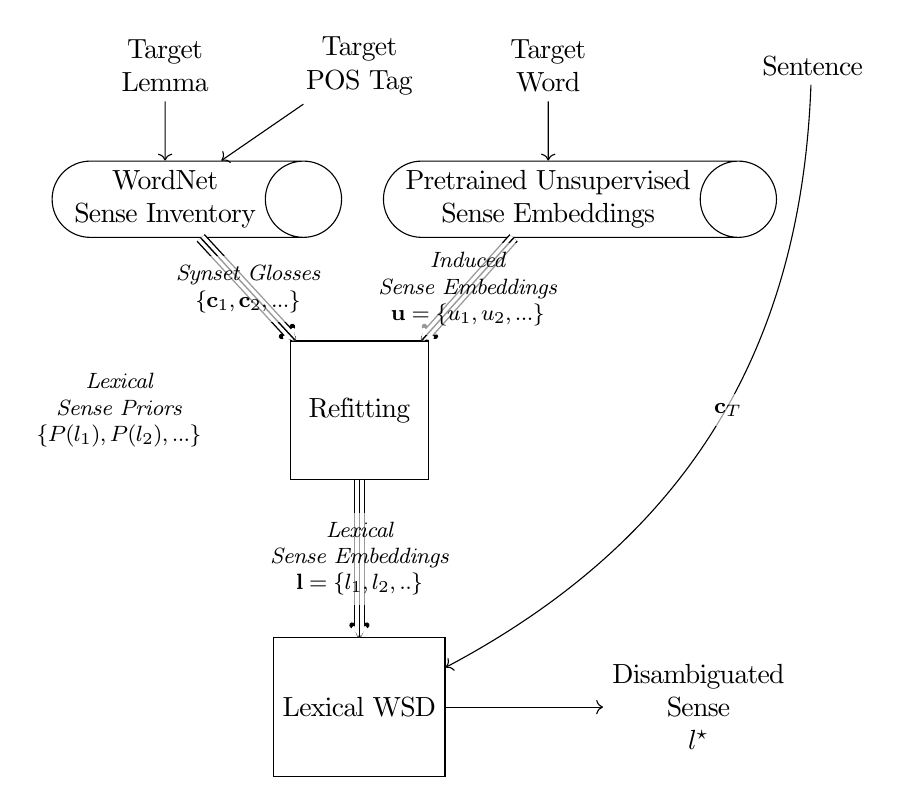
\begin{tikzpicture}[align=center]

\node[input](lemma){Target\\Lemma};
\node[input, right = 1\xunit of lemma](POS){Target\\POS Tag};
\node[input, right = 1\xunit of POS](word){Target\\ Word};
\node[datastore, below=0.75 of lemma](wordnet){WordNet \\Sense Inventory};

\node[datastore, below=0.75 of word](embeddings) {Pretrained Unsupervised \\ Sense Embeddings};
\node[proc, below=3 of POS] (refitting) {Refitting};

\node[proc, below = 2 of refitting] (WSD) {Lexical WSD};
\node[input, right = 2\xunit of word] (sentence) {Sentence};

\node[input, right = 2\xunit of WSD] (output){Disambiguated\\ Sense\\ $l^\star$};


\draw[link] (lemma) edge (wordnet);
\draw[link] (POS) edge (wordnet);
\draw[link] (word) edge (embeddings);

\draw[multi] (wordnet) -> (refitting) node[midway, labe]{Synset Glosses \\ $\{\c_1,\c_2,...\}$};
\draw[multi] (embeddings) -> (refitting) node[midway, labe]{Induced \\ Sense Embeddings \\$\u=\{u_1,u_2,...\}$};;

\draw[multi] (refitting) -> (WSD) node[midway, labe]{Lexical\\ Sense Embeddings\\ $\l=\{l_1,l_2,..\}$};
\draw[link] (sentence) edge[bend left] (WSD);
%\draw[multi, bend right] (wordnet) -> (WSD);
\triplearrow{arrows={-Implies}}{(wordnet) to[bend right] (WSD)};
\node[labe, left = 1\xunit of refitting] {Lexical\\Sense Priors\\$\{P(l_1), P(l_2),...\}$}; %hack cos benlines don't label right
\node[labe, right = 3.5\xunit of refitting] {$\c_T$}; %hack cos benlines don't label right

\draw[link] (WSD) -> (output);

\end{tikzpicture}
\end{document}
	\end{adjustbox}
	\caption{\pdfcomment{This figure is a placeholder} block diagram for performing WSD using refitting \label{WSDBlock}} 
\end{figure}
Once refitting has been used to create sense vectors that are matched to lexical word senses, we would like to use them to perform word sense disambiguation. This would show whether or not the refitted embeddings are capturing the lexical information. In this section we refer to the lexical word sense disambiguation problem -- to take a word and find its dictionary sense; whereas the methods discussed in \Cref{eq:generalwsd} and \Cref{eq:generalwsdsmoothed} consider the more general word sense disambiguation problem, as applicable to disambiguate to lexical word senses, or induced word senses, depending on the inputs.
Our overall process must use both: first disambiguating the induced senses as part of refitting, then using the refitted sense vectors to find the most likely dictionary sense.
The overall process is shown in \Cref{WSDBlock}.

First, we perform refitting, to transform the induced sense vectors, into lexical sense vectors.
We use the targeted word's lemma (i.e. base form), and part of speech (POS) tag to retrieve all possible definitions of the word (Glosses) from WordNet; there is one gloss per sense. These glosses are used as the example sentence to perform refitting. By applying refitting to the unsupervised senses using these example sentence, as discussed in \Cref{refitting}, we find embeddings, $\l=\{l_1,..., l_{n_l}\}$ for each of the lexical word senses. These lexical word senses are still supported by the language model, which means one can apply the general WSD method to determine the posterior probability of a word sense, given an observed context. 

When given a sentence $\c_{T}$, containing a target word to be disambiguated, 
the probability of each lexical word sense $P(l_i \mid \c_{T})$, can be found using \Cref{eq:generalwsd} (or the smoothed version \Cref{eq:generalwsdsmoothed}), over the lexically refitted sense embeddings. Then selecting the correct sense is simply selecting the most likely sense:
\begin{equation}
\begin{aligned}\label{eq:lexicalwsd}
l^\star (\l, \c_T) &= \argmax_{\forall l_i \in \l} P(l_i|\c_T) \\
&= \argmax_{\forall l_i \in \l} \frac{P(\c_T \mid l_i)P(l_i)}{\sum_{\forall l_j \in \l} P(\c_T \mid l_j)P(l_j)}
\end{aligned}
\end{equation}

WordNet glosses are less than ideal examples sentences. As well as being definitions, rather than examples of use, they are shared across many words. Each lexical word sense shares its gloss with the rest of the set of synonymous senses from different words (synsets). Similarly as the synsets are defined per lemma (base word), the different lexeme (tenses and other variants) of a word also share the same example sentence. However, in both cases this does not mean that their refitted sense vectors are equal (though they are likely to be similar). When refitting the different lexemes correspond to different induced sense vectors, and these as well as the probabilities of the examples, are the contributing factors to the refitting sum. The limitations of the glosses does not prevent our refitting system from functioning.

\subsection{Lexical Sense Prior}
WordNet includes frequency counts for each word sense based on Semcor \textcite{tengi1998design}. These form a prior for $P(l_i)$.

However, Semcor is not an immense corpus, being only a subset of the Brown corpus. The comparatively small size of Semcor means that many word senses do not occur at all. As counted by WordNet 2.1, there are counts for just  36,973 word senses, out of the total 207,016 senses in WordNet; i.e. 82\% of all senses have no count information.

An additional issue is that Semcor's underling texts from Brown are now significantly ageing. They are all from 1961 \cite{francis1979brown} -- it is not unreasonable to suggest that the frequency of word sense use has changed significantly in the last half century.

Never-the-less, the word count is the best prior readily available. Given the highly unbalanced distribution of sense occurrence a uniform prior would not be a reasonable approximation.
We apply add-one smoothing to find the prior, to remove any zero counts.
This is in addition to using our proposed geometric smoothing as an optional part of the general WSD.
Geometric smoothing which serves a different (but related) purpose, of decreasing the sharpness of the likelihood function -- not of removing impossibilities from the prior.

\subsection {Experimental Setup}
The WSD performance was evaluated on the SemEval 2007 Task 7. 
WordNet 2.1, was used as the sense inventory.
All glosses were converted to lower case, when used as as the example sentences in the refitting step. They were not clipped to a window around the target word, as the target word often does not occur at all in the gloss; and the glosses are already close to the correct size.

We used the weighted mapping method of Agirre et al \parencite{agirre2006}, (see \Cref{mapping}) as a baseline; to compare an alternative method for using WSI senses for WSD.
When estimating the sense mapping weights we used both of the all-words-annotated subcorpora (Brown1 and Brown2) of SemCor as the mapping corpus.
While evaluating the map, we do clip to a 10 word context window for each word to be disambiguated.

The second baseline we use is the Most Frequent Sense (MFS). This method always disambiguates any word as having its  most common meaning. Due to the power law distribution of word senses, this is an effective heuristic \parencite{Kilgarriff2004}.

We also evaluted the performance of the mapping baseline, and the Greedy embedding method with a backoff to the MSF. When a method is unable to determine the word sense, the method can report the MFS instead of returning no result (a non-attempt). For embedding methods, this occurs when a polysemous word has only one (or zero) sense embeddings trained. For the mapping method it occurs when the word does not occur in the mapping corpus. We do not report the results for AdaGram with MSF backoff, as it was trained with a large enough vocabulary, that it has almost complete coverage.

\subsection{Word Sense Disambiguation Results} \label{WSDtask}
\pgfplotstableset{
	nhundred/.style={
 		numeric type,
		precision=3,
		fixed zerofill=true,
		column type=r
%		preproc/expr={100*##1}
	}
}
\begin{table}
	\begin{adjustbox}{max width=\columnwidth}
		\pgfplotstabletypeset[col sep=comma, header=has colnames, string type,
		every head row/.style={after row = {\toprule}},
%
		columns/Method/.style={ 
			column type=l
		},
%
		columns/Attempted/.style={ 
			column type=r
		},
%
		columns/F1/.style={nhundred},
		columns/Precision/.style={nhundred},
		columns/Recall/.style={nhundred},
%
		every row 0 column F1/.style={
			postproc cell content/.style={
				@cell content/.add={$\bf}{$}
			}
		}
%				
		]{semeval2007t7-short.csv}
	\end{adjustbox}

	\caption{Results on SemEval 2007 Task 7 -- course-all-words disambiguation.
	The \emph{-S} marks results using geometric smoothing.
	the \emph{\textasteriskcentered } marks results with backoff.
	} \label{samevalres}
\end{table}

The results of employing our method for WSD , are shown in \Cref{samevalres}. Our results with AdaGram when using refitting with geometric smoothing, output perform the MSF baseline -- noted as a surprisingly hard baseline to beat \parencite{Chen2014}. Our results with the Greedy Embeddings, when using MSF backoff also exceed this baseline.

We found that the mapping method\parencite{agirre2006}  was not up to the task of mapping unsupervised senses to supervised senses, on this large scale task. There is simply not enough data in SemCor to allow it to properly estimate the mapping weights. The Refitting method worked significantly better. Though refitting is only usable for language model based sense embeddings, where as the mapping method is suitable for all WSI systems.

While not directly comparable due to the difference in training data, we note that our Refitted results, are similar in performance, as measured by F1 score, to the results reported by Chen et al \parencite{Chen2014}.
AdaGram with smoothing, and Greedy embeddings with backoff have close to the same result as reported for L2R with backoff -- with the AdaGram slightly better and the Greedy embeddings slightly worse. They are exceeded by the best method reported in that paper: S2C method with backoff.

Our results are not strong enough for Refitted AdaGram to be used as a WSD method on its own, but do demonstrate that the senses found by refitting are capturing the information from lexical senses. We have demonstrated that it is now able to perform WSD, which was not possible with the unsupervised senses. 

\section{Conclusion}\label{conclusion}

We have presented a new method for taking unsupervised word embeddings, and adapting them to align to particular given uses. This refitting method thus allows us to find word sense embeddings with known meaning. This method can be seen as a one shot learning task, where only a single labelled example of each class is available for training.

We showed how our method could be used to create embeddings to evaluate the similarity of words, given their contexts. This in itself is a new similarity measuring method, RefittedSim.  RefittedSim has time complexity is $O(n \times n^\prime)$ less than that of AvgSimC. The performance of RefittedSim on AdaGrams is comparable to the results reported by the proposers of other sense embeddings techniques using AvgSimC.

We also demonstrated how similar refitting principles could be used to create a set of vectors that are aligned to the meanings in a sense inventory, such as WordNet. We showed how this could be used for word sense disambiguation. On this difficult task, it performed marginally better than the MFS baseline, and significantly better than a general mapping method used for working with WSI senses with lexical WSD tasks,

As part of our method for refitting the sense embeddings to their new senses, we presented a geometric smoothing to avoid overly certain decisions caused by limited training data.
We show that this improves the results for the similarity task with both RefittedSim, and with AvgSimC; and also that it improves the WSD results.

Our refitting method allows bridging between the vector space representation of meaning, and the traditional discrete lexical representation. More generally it allows a sense embedding to be created to model the meaning a word in any given sentence.

\newpage
\microtypesetup{protrusion=false}
\printbibliography

\end{document}
